\subsection{\textit{Partitioning} Basis Data}

\textit{Partitioning} (atau \textit{sharding}) merupakan sebuah cara untuk membagi basis data yang besar menjadi bagian-bagian yang lebih kecil \parencite{dataIntensiveApplications}. Beberapa partisi dapat disimpan pada \textit{node} yang berbeda, sehingga dataset yang besar dapat didistribusikan pada beberapa media penyimpanan. Selain itu, beban \textit{query} juga dapat didistribusikan kepada beberapa mesin yang berbeda.

\textit{Partitioning} dapat dibagi menjadi dua, yaitu \textit{horizontal partitioning} yang membagi data berdasarkan \textit{rows} dan \textit{vertical partitioning} yang membagi data berdasarkan kolom.

Tujuan dari pempartisian data adalah untuk menyebarkan data dan beban secara adil kepada \textit{nodes} yang berbeda. Untuk itu, pendekatan untuk membagi data juga menjadi hal yang penting dalam partisi data. Berikut adalah beberapa pendekatan yang umum digunakan:

\begin{enumerate}
    \item Partisi berdasarkan \textit{keys}, seperti judul buku yang berawalan A-E, F-J, dan seterusnya. Meskipun begitu, perlu diiperhatikan apakah distribusi \textit{keys} tersebar secara merata.
          \begin{figure}[ht]
              \centering
              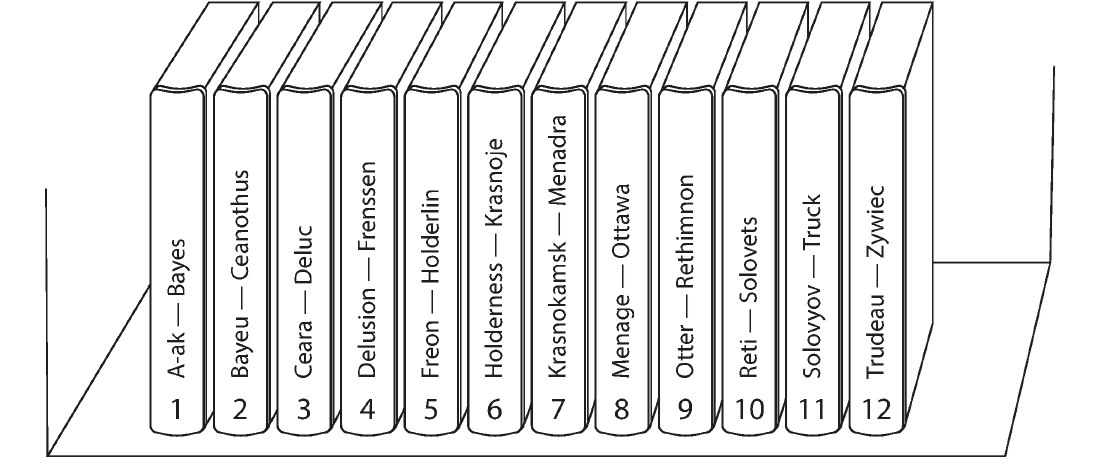
\includegraphics[width=0.8\textwidth]{resources/chapter-2/partition-by-key-range.png}
              \caption{\textit{Partition by key range \parencite{dataIntensiveApplications}}}
              \label{fig: partition-by-key-range}
          \end{figure}

    \item Partisi berdasarkan \textit{hash of key}. Fungsi hash yang baik dapat mengubah distribusi \textit{keys} yang \textit{skewed} menjadi merata.
          \begin{figure}[ht]
              \centering
              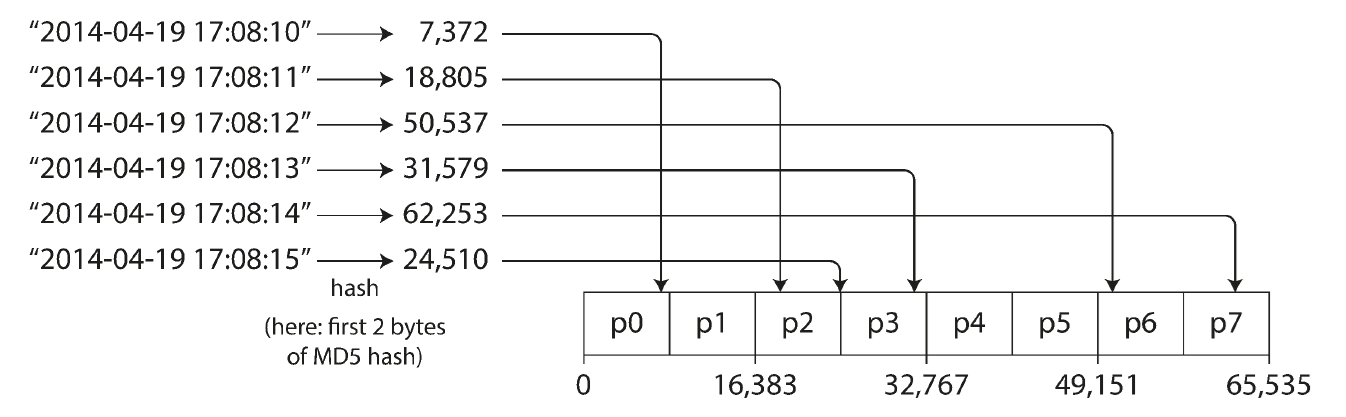
\includegraphics[width=0.8\textwidth]{resources/chapter-2/partition-by-hash.png}
              \caption{\textit{Partition by hash \parencite{dataIntensiveApplications}}}
              \label{fig:partition-by-hash}
          \end{figure}

\end{enumerate}